\chapter{Referencial Teórico}

\section{Histograma}

\section{Gradientes}

Um dos mais importantes processos no processamento de uma imagem é a sua segmentação. A segmentação consiste em subdividir a imagem em regiões ou objetos de interesse. O nível de segmentação depende do problema a ser resolvido e é comumente baseado em duas propriedades do valor da intensidade: descontinuidade e similaridade. A primeira consiste em particionar uma imagem baseado nas mudanças abruptas na intensidade, como por exemplo as bordas de um objeto. Já na segunda, é feito o agrupamento de uma região baseado em sua similaridade com outras partes da imagem, como cor ou nível de intensidade.

Gonzales define borda como sendo um conjunto de pixeis conectados  presente na fronteira entre duas regiões. E conclui que a magnitude da primeira derivada pode ser usada para detectar da borda em um ponto da imagem.

A derivada de primeira ordem de uma imagem digital pode ser aproximada no gradiente 2D. O gradiente de uma imagem \(f(x,y)\) no ponto \((x,y)\) e definido como um vetor

\begin{equation}
\nabla \mathbf{f}(x,y) = 
\begin{bmatrix}
G_x \\ G_y
\end{bmatrix} =
\begin{bmatrix}
\dfrac{ \partial f}{\partial x} 
\\[2ex]
\dfrac{ \partial f}{\partial y}
\end{bmatrix}
\end{equation}

cuja magnitude é definida como \(\nabla f\), onde

\begin{equation}
\nabla f = mag(\nabla \mathbf{f}) = 
\begin{bmatrix}
G_x^2 + G_y^2
\end{bmatrix}^{1/2}
\end{equation}

e a direção do vetor \(\alpha(x,y)\) sendo definida como

\begin{equation}
\alpha(x,y) = tan^{-1}
\left (
\dfrac{G_y}{G_x}
\right)
\end{equation}

onde o ângulo é medido em referência ao eixo \(x\). A direção de uma borda no ponto \((x,y)\) é perpendicular à direção do vetor gradiente no ponto.

O cálculo dessas derivadas podem ser implementados usando máscaras como o da figura \ref{fig:gradiente_mascara}. A máscara é aplicada em cada pixel da imagem e um novo valor é calculado conforme a equação \ref{eq:gradiente_mascara}.

\begin{equation}
R = w_1 z_1 + w_2 z_2 + w_3 z_3 + ... +w_9 z_9 = \sum_{i=1}^{9}{w_iz_i}
\label{eq:gradiente_mascara}
\end{equation}

\begin{figure}
\begin{center}
\begin{tabular}{| l |c | r |}
\hline
\(w_1\) & \(w_2\) & \(w_3\) \\ \hline
\(w_4\) & \(w_5\) & \(w_6\) \\ \hline
\(w_7\) & \(w_8\) & \(w_9\) \\ \hline
\end{tabular}
\end{center}
\caption{Exemplo de máscara 3x3}
\label{fig:gradiente_mascara}
\end{figure}

\begin{figure}
	\centering
	\begin{subfigure}[b]{0.3\textwidth}
	\begin{center}
		\begin{tabular}{| l | c | r |}
		\hline
		-1 & -1 & -1 	\\ \hline
		0 & 0 & 0 		\\ \hline
		1 & 1 & 1 		\\ \hline
		\end{tabular}
		\begin{tabular}{| l | c | r |}
		\hline
		-1 & 0 & 1	 	\\ \hline
		-1 & 0 & 1 		\\ \hline
		-1 & 0 & 1 		\\ \hline
		\end{tabular}
		\caption{Máscara Prewitt}
		\label{fig:gradiente_prewitt}
	\end{center}
	\end{subfigure}
	\begin{subfigure}[b]{0.3\textwidth}
	\begin{center}
		\begin{tabular}{| l | c | r |}
		\hline
		-1 & -2 & -1 	\\ \hline
		0 & 0 & 0 		\\ \hline
		1 & 2 & 1 		\\ \hline
		\end{tabular}
		\begin{tabular}{| l | c | r |}
		\hline
		-1 & 0 & 1	 	\\ \hline
		-2 & 0 & 2 		\\ \hline
		-1 & 0 & 1 		\\ \hline
		\end{tabular}
		\caption{Máscara Sobel}
		\label{fig:gradiente_sobel}
	\end{center}
	\end{subfigure}
\end{figure}

Nas figuras \ref{fig:gradiente_prewitt} e \ref{fig:gradiente_sobel} temos dois exemplo das máscaras mais utilizadas para cálculo de gradiente. Na figura \ref{fig:gradientes} podem ver o resultado das máscaras em uma imagem de uma pose de mão aberta feita por uma câmera infra vermelha.

\begin{figure}
    \centering
    \begin{subfigure}[b]{0.3\textwidth}
        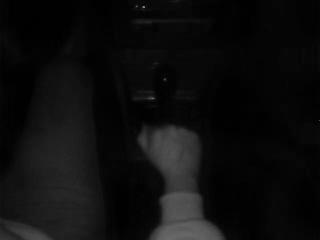
\includegraphics[width=\textwidth]{image/gradiente_original.jpg}
        \caption{Original}
        \label{fig:gradiente_original}
    \end{subfigure}%
    ~ %add desired spacing between images, e. g. ~, \quad, \qquad, \hfill etc.
      %(or a blank line to force the subfigure onto a new line)
    \begin{subfigure}[b]{0.3\textwidth}
        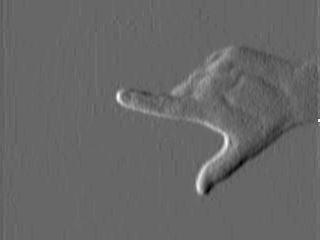
\includegraphics[width=\textwidth]{image/gradiente_prewitt_gx.jpg}
        \caption{Prewitt Gx}
        \label{fig:gradiente_gx}
    \end{subfigure}
    ~ %add desired spacing between images, e. g. ~, \quad, \qquad, \hfill etc.
      %(or a blank line to force the subfigure onto a new line)
    \begin{subfigure}[b]{0.3\textwidth}
        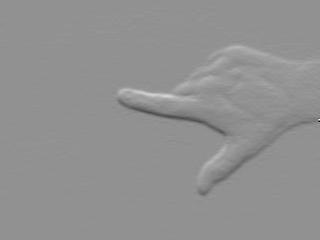
\includegraphics[width=\textwidth]{image/gradiente_prewitt_gy.jpg}
        \caption{Prewitt Gy}
        \label{fig:gradiente_gy}
    \end{subfigure}
    \begin{subfigure}[b]{0.3\textwidth}
        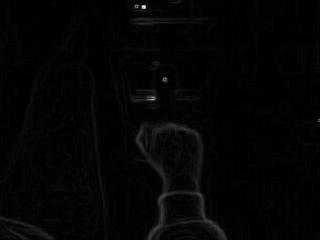
\includegraphics[width=\textwidth]{image/gradiente_prewitt_mag.jpg}
        \caption{Prewitt Gmag}
        \label{fig:gradiente_gmag}
    \end{subfigure}%
    ~ %add desired spacing between images, e. g. ~, \quad, \qquad, \hfill etc.
      %(or a blank line to force the subfigure onto a new line)
    \begin{subfigure}[b]{0.3\textwidth}
        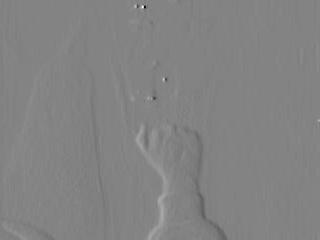
\includegraphics[width=\textwidth]{image/gradiente_sobel_gx.jpg}
        \caption{Sobel Gx}
        \label{fig:gradiente_gx}
    \end{subfigure}
    ~ %add desired spacing between images, e. g. ~, \quad, \qquad, \hfill etc.
      %(or a blank line to force the subfigure onto a new line)
    \begin{subfigure}[b]{0.3\textwidth}
        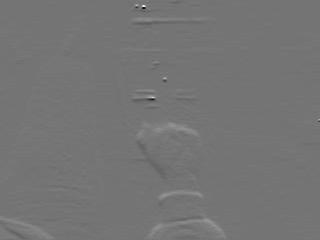
\includegraphics[width=\textwidth]{image/gradiente_sobel_gy.jpg}
        \caption{Sobel Gy}
        \label{fig:gradiente_gy}
    \end{subfigure}
    \begin{subfigure}[b]{0.3\textwidth}
        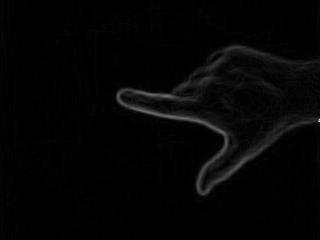
\includegraphics[width=\textwidth]{image/gradiente_sobel_mag.jpg}
        \caption{Sobel Gmag}
        \label{fig:gradiente_gmag}
    \end{subfigure}
    \caption{Gradientes}\label{fig:gradientes}
\end{figure}

\section{Norma}

Norma é uma função que atribui um tamanho de valor positivo e diferente de zero para um vetor em um espaço vetorial.

A função norma deve satisfazer algumas propriedades de escalabilidade e aditividade.
Sendo um espaço vetorial \(V\) em um sub corpo \(F\) de números complexos, a norma em \(V\) é uma função \(p:\rightarrow \mathbf{R}\) com as seguintes propriedades.

\begin{itemize}
\item \( p(a\mathbf{v}) = |a|p(\mathbf{v}) \)
\item \( p(\mathbf{u + v}) \leq p(\mathbf{u}) + p(\mathbf{v}) \)
\item Se \( p(\mathbf{v}) = 0 \) então \(\mathbf{v}\) é o vetor zero.
\end{itemize}


\section{Histograma orientado a gradientes}

HOG (Histogram of oriented gradients) é um descritor computado a partir dos gradientes da imagem, podemos defini-lo com sendo uma informação estatística do gradiente e intensidade de uma área. Suas principais propriedades são a robustez para pequenas variações nos locais dos contornos, direções e variações significativas na iluminação e cor.

O HOG proposto por Dalal \cite{dalal} possui a seguinte parametrização conforme tabela \ref{table:dlal_hog}.

\todo {Ver \cite{ref16} para uma descrição do HOG}

\begin{table}[h]
\centering
\begin{tabular}{|c|c|}
\hline Cor & RGB sem correção de gamma \\ 
\hline Gradiente & [-1, 0, 1] sem smoothing \\ 
\hline Bins & 9 \\
\hline Orientação & 0 à 180 \\
\hline Tamanho do bloco & 16x16 pixels \\
\hline Tamanho da célula & 8x8 pixels \\
\hline Janela Gaussian & 8 pixel \\
\hline Normalização & L2-Hys \\
\hline Janela de detecção & 64x128 \\
\hline 
\end{tabular} 
\caption{Parâmetros do HOG otimizado por Dalal}
\label{table:dlal_hog}
\end{table}

\subsection{Normalização Gamma/Cor}

\subsection{Gradientes}

O gradiente é computado da seguinte maneira.

\[G_{x}(x,y) = H(x+1, y) - H(x-1, y)\]
\[G_{y}(x,y) = H(x, y+1) - H(x, y-1)\]

Aqui, \(G_{x}\) representa o gradiente horizontal e \(G_{y}\) o gradiente vertical de cada pixel na imagem (ou em um pedaço da imagem).

Depois calculamos a intensidade e orientação de cada ponto da imagem.

\[G(x,y) = \sqrt{G_{x}(x,y)^{2} + G_{y}(x,y)^{2}}\]
\[\alpha (x,y) = tan^{-1} \left(\frac{G_{y}(x,y)}{G_{x}(x,y)}\right)\]

\subsection{Classificação dos ângulos}

Depois dos cálculos do gradiente, a imagem é então dividida em pequenos retângulos (células). Para cada célula, um histograma é calculado. Esse histograma é a coleção dos ângulos dos vetores de gradiente de cada pixel que compõe a célula. Os ângulos podem ser agrupados variando de 0 à 360 graus ou de 0 à 180 graus. O número de grupos em cada histograma é 20.

\[
V_{k}(x,y) = \left\{\begin{matrix}
G(x,y), \alpha (x,y)  \in bin_{k}\\ 
0, \alpha (x,y) \notin bin_{k}
\end{matrix}\right. k \in (1,20)
\]

\subsection{Normalização em blocos}

Dalal extraiu o HOG em blocos de tamanho 16x16 e dividiu cada bloco em 4 células. Para eliminar os impactos da luminosidade, foi feito uma normalização em cada bloco.

\[
f(C_{i},k) = \frac
{\sum_{(x,y) \in C_i}V_k(x,y) + \varepsilon}
{\sum_{(x,y) \in B}V_k(x,y) + \varepsilon}
\]

\(f(C_i,k)\) é a proporção do valor do gradiente acumulado do kth bin no bloco que contém a célula \(C_i\). O \(\varepsilon\) é um valor bem pequeno para eliminar os denominadores zeros.

Depois cada histograma é concatenado, formando um vetor único de características.

%Parâmetros:
%
%- imagens tons de cinza (talvez comparar com imagens binárias);
%- filtros: sem filtro / gaussiano;
%- Máscara para cálculo do gradiente: [-1 0 +1]
%- Angulos: 0-180 ou 0-360
%- Numero de bins
%- Voted bin
%- Normalização em blocos
%- Numero de celulas
%- Numero de blocos


\chapter{XXX}

\section{Construção da câmera infra vermelha}

A câmera utilizada nessa aplicação tem que ser capaz de capturar imagens nas mais diversas condições de luminosidade. Temos o caso, por exemplo, de um dia de sol cuja intensidade de luz é bem alta. Até o ponto onde não há luz nenhuma.
Nesses casos é necessário uma iluminação própria, mas ao mesmo tempo, não pode atrapalhar o motorista. Por isso, a iluminação infra vermelha é muito utilizada. O custo é baixo e não interfere em nada no ambiente. O maio contratempo desse tipo de iluminação é que se perde toda a informação de cor.
Para gerar a base de dados para o nosso estudo, utilizamos uma câmera normal de mercado, modificada para receber a luz infra vermelha e colocamos LEDs de infra vermelho para fazer a iluminação.

\todo{Colocar a referencia}
\todo{Adicionar o espectro do sol}

\begin{figure}[ht!]
\centering
\fbox{
  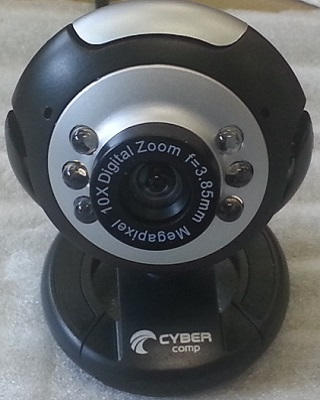
\includegraphics[width=0.3\textwidth]{image/webcam01.jpg}
  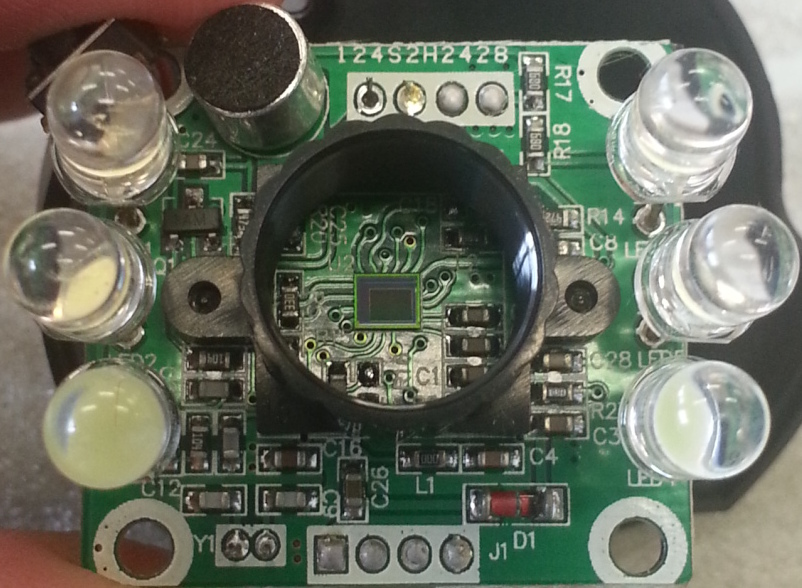
\includegraphics[width=0.3\textwidth]{image/webcam02.jpg}}
  \caption{Webcam utilizada na aquisição das imagens sem nenhuma modificação}
  \label{fig:camera_01}
\end{figure}

Na figura \ref{fig:camera_01} temos a câmera utilizada para a aquisição das imagens. Nesse momento a câmera ainda não foi modificada. Essa câmera portanto ainda possui um filtro de luz infra vermelha e os LEDs de iluminação são LEDs brancos.

A principal modificação a ser feita nesse tipo de câmera é retirar o filtro infra vermelho. Esse filtro é uma placa de vidro localizado atrás da lente. Na figura \ref{fig:camera_02} temos uma foto das lentes ainda com o filtro e depois já com o filtro retirado. E preciso também substituir os LEDs atuais, que são LEDs brancos, para LEDs infra vermelho de 950nm.

\begin{figure}[ht!]
\centering
\fbox{
  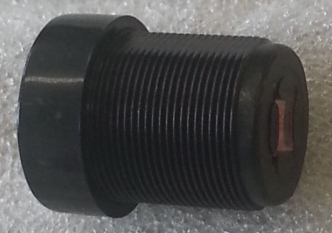
\includegraphics[width=0.3\textwidth]{image/webcam03.jpg}
  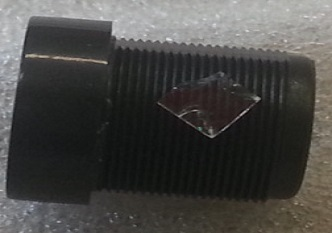
\includegraphics[width=0.3\textwidth]{image/webcam05.jpg}}
  \caption{Lentes com o filtro infra vermelho localizado na parte traseira}
  \label{fig:camera_02}
\end{figure}

